\documentclass[aspectratio=169]{beamer}

\mode<presentation>

\usepackage[utf8]{inputenc}
\usepackage[T1]{fontenc}	%makes å,ä,ö etc. proper symbols
\usepackage{amsmath}
\usepackage{graphicx}
\usepackage{xcolor}
\usepackage{listings}
\usepackage{multicol}
\usepackage{hyperref}


\definecolor{LundaGroen}{RGB}{00,68,71}
\definecolor{StabilaLila}{RGB}{85,19,78}
\definecolor{VarmOrange}{RGB}{237,104,63}

\definecolor{MagnoliaRosa}{RGB}{251,214,209}
\definecolor{LundaHimmel}{RGB}{204,225,225}
\definecolor{LundaLjus}{RGB}{255,242,191}

\usefonttheme{serif}
\usetheme{malmoe}
\setbeamercolor{palette primary}{bg=VarmOrange}
\setbeamercolor{palette quaternary}{bg=LundaGroen}
\setbeamercolor{background canvas}{bg=LundaLjus}
\setbeamercolor{structure}{fg=LundaGroen}

\usepackage[many]{tcolorbox}

\newtcolorbox{cross}{blank,breakable,parbox=false,
  overlay={\draw[red,line width=5pt] (interior.south west)--(interior.north east);
    \draw[red,line width=5pt] (interior.north west)--(interior.south east);}}



\lstset{language=Python} 
\lstset{%language=[LaTeX]Tex,%C++,
    morekeywords={PassOptionsToPackage,selectlanguage,True,False},
    keywordstyle=\color{blue},%\bfseries,
    basicstyle=\small\ttfamily,
    %identifierstyle=\color{NavyBlue},
    commentstyle=\color{red}\ttfamily,
    stringstyle=\color{VarmOrange},
    numbers=left,%
    numberstyle=\scriptsize,%\tiny
    stepnumber=1,
    numbersep=8pt,
    showstringspaces=false,
    breaklines=true,
    %frameround=ftff,
    frame=single,
    belowcaptionskip=.75\baselineskip,
	tabsize=4,
	backgroundcolor=\color{white}
    %frame=L
}

\begin{document}

\lstset{literate=
  {á}{{\'a}}1 {é}{{\'e}}1 {í}{{\'i}}1 {ó}{{\'o}}1 {ú}{{\'u}}1
  {Á}{{\'A}}1 {É}{{\'E}}1 {Í}{{\'I}}1 {Ó}{{\'O}}1 {Ú}{{\'U}}1
  {à}{{\`a}}1 {è}{{\`e}}1 {ì}{{\`i}}1 {ò}{{\`o}}1 {ù}{{\`u}}1
  {À}{{\`A}}1 {È}{{\'E}}1 {Ì}{{\`I}}1 {Ò}{{\`O}}1 {Ù}{{\`U}}1
  {ä}{{\"a}}1 {ë}{{\"e}}1 {ï}{{\"i}}1 {ö}{{\"o}}1 {ü}{{\"u}}1
  {Ä}{{\"A}}1 {Ë}{{\"E}}1 {Ï}{{\"I}}1 {Ö}{{\"O}}1 {Ü}{{\"U}}1
  {â}{{\^a}}1 {ê}{{\^e}}1 {î}{{\^i}}1 {ô}{{\^o}}1 {û}{{\^u}}1
  {Â}{{\^A}}1 {Ê}{{\^E}}1 {Î}{{\^I}}1 {Ô}{{\^O}}1 {Û}{{\^U}}1
  {œ}{{\oe}}1 {Œ}{{\OE}}1 {æ}{{\ae}}1 {Æ}{{\AE}}1 {ß}{{\ss}}1
  {ű}{{\H{u}}}1 {Ű}{{\H{U}}}1 {ő}{{\H{o}}}1 {Ő}{{\H{O}}}1
  {ç}{{\c c}}1 {Ç}{{\c C}}1 {ø}{{\o}}1 {å}{{\r a}}1 {Å}{{\r A}}1
  {€}{{\euro}}1 {£}{{\pounds}}1 {«}{{\guillemotleft}}1
  {»}{{\guillemotright}}1 {ñ}{{\~n}}1 {Ñ}{{\~N}}1 {¿}{{?`}}1
}

% NEW COMMANDS
\newcommand{\fortt}{\texttt{for}}
\newcommand{\whilett}{\texttt{while}}
\newcommand{\iftt}{\texttt{if}}

\AtBeginSection[ ]
{
\begin{frame}{Outline}
    \tableofcontents[currentsection]
\end{frame}
}

\title{GUI 3}
\date{vt 25}
\author{Programmering 2}

\maketitle

\tableofcontents

\section{Widgets}

\subsection{Tidigare widgets}

\begin{frame}[fragile]
	\frametitle{Widgets}
	\framesubtitle{tidigare widgets}
	
	Vi har hittills gått igenom följande widgets:
	
	\begin{itemize}
		\item \lstinline!Label(root, text='')! skapar en text-widget
		\item \lstinline!Button(root, text='', command=funk)! skapar en knapp-widget. Tänk på att funktionen ska skrivas utan avslutande paranteser!
		\item \lstinline!Entry(root)! ett fält användaren kan fylla i
	\end{itemize}	
	
	\texttt{root} är i alla tre fallen variabeln som håller vårt fönster (\lstinline!root = tk.Tk()!)
	
\end{frame}

\subsection{Widgeten Listbox}

\begin{frame}[fragile]
	\frametitle{Widgets}
	\framesubtitle{Listbox}
	
	Till det här passet lägger vi till en ny widget: Listbox
	
	\begin{lstlisting}
import tkinter as tk

root = tk.Tk()
box = tk.Listbox(root)
text1 = tk.Label(root, text="Bara för att visa")
text2 = tk.Label(root, text="Bara för att visa")

text1.pack()
box.pack()
text2.pack()

root.mainloop()
	\end{lstlisting}
	
\end{frame}

\begin{frame}
	\frametitle{Widgets}
	\framesubtitle{Listbox}
	\centering
	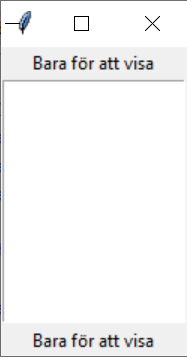
\includegraphics[]{listbox-tom.png}
\end{frame}

\begin{frame}[fragile]
	\frametitle{Widgets}
	\framesubtitle{Listbox}
	
	\begin{itemize}
		\item För att lägga till i listan skriver du: \lstinline!box.insert(tk.END, "Text")!
		\item \lstinline!tk.END! anger att vi ska lägga till sist i listan
	\end{itemize}
	
	\begin{center}
		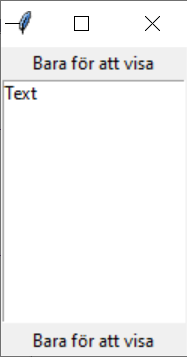
\includegraphics[width=.175\linewidth]{list-box-text.png}
	\end{center}
\end{frame}

\begin{frame}[fragile]
	\frametitle{Widgets}
	\framesubtitle{Listbox}
	
	\begin{itemize}
		\item För att läsa in vilka rader i listan som är markerade skriver du \lstinline!selection = box.curselection()!
		\item Detta sparar en lista med alla index som är markerade i variabeln \lstinline!selection!.
		\item Vill du bara ha den första som är markerad (eller enda) kan du skriva \lstinline!selection[0]! eller \lstinline!selection = box.curselection()[0]!
	\end{itemize}
	
\end{frame}

\section{Knyta samman}

\begin{frame}[fragile]
	\frametitle{Knyta samman}
	\framesubtitle{Klasser}
	
	\begin{itemize}
		\item När man vill göra ett större program är det ofta användbart att använda en klass för att skapa fönstret:
		\item En fördel med detta är att man kan komma åt alla instansvariabler i de olika metoderna fritt. 
	\end{itemize}
	
	\begin{lstlisting}
import tkinter as tk
class App():
    def __init__(self):
        self.root = tk.Tk()
        self.root.mainloop()
app = App()
	\end{lstlisting}
\end{frame}

\begin{frame}[fragile]
	\frametitle{Knyta samman}
	\framesubtitle{Ett program som läser in information från en fil}
	
	\begin{lstlisting}
import tkinter as tk
class App():
    def __init__(self):
        self.root = tk.Tk() # Skapa fösntret
        # Hantera widgets
        self.create_widgets()
        self.place_widgets()
        
        self.root.mainloop() # Håll programmet vid liv
	\end{lstlisting}
	
\end{frame}

\begin{frame}[fragile]
	\frametitle{Knyta samman}
	\framesubtitle{Ett program som läser in information från en fil}
	
	\begin{lstlisting}
	def create_widgets(self):
	    """
	    Metod som skapar alla widgets
	    """
	    self.file_entry = tk.Entry(self.root)
	    self.load_file_button = tk.Button(self.root, 
	        text="Ladda fil", command=self.load_file)
	    self.text_label = tk.Label(self.root, text="")
	\end{lstlisting}
	
\end{frame}

\begin{frame}[fragile]
	\frametitle{Knyta samman}
	\framesubtitle{Ett program som läser in information från en fil}
	
	\begin{lstlisting}
	def place_widgets(self):
		"""
		Metod som placerar ut alla widgets
		"""
		self.file_entry.grid(row=0, column=0)
		self.load_file_button.grid(row=0, column=1)
		self.text_label.grid(row=1,column=0, columnspan=2)
	\end{lstlisting}
	
\end{frame}

\begin{frame}[fragile]
	\frametitle{Knyta samman}
	\framesubtitle{Ett program som läser in information från en fil}
	
	\begin{lstlisting}
	def load_file(self):
	    """
	    Metod som läser in en angiven fil och skriver ut första raden
	    """
	    file_name = self.file_entry.get()
	    try:
	        with open(file_name, encoding="utf-8") as f:
	            self.data = f.readlines()
       except FileNotFoundError: # Om filen inte finns
           return # Avbryt det vi gör
       self.text_label["text"] = self.data[0]

app = App() # Kör appen
	\end{lstlisting}
	
\end{frame}

\begin{frame}[fragile]
	\frametitle{Knyta samman}
	\framesubtitle{Ett program som läser in information från en fil}
	
	\centering
	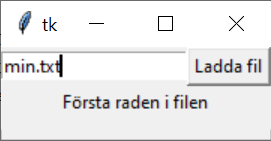
\includegraphics{exempel.png}
	
\end{frame}

\begin{frame}
	\frametitle{Knyta samman}
	\framesubtitle{Ett program som läser in information från en fil}
	
	\centering
	
	\begin{tabular}{|l|}
		\hline
		\textbf{App()} \\ \hline
		file\_entry: tk.Entry\\
		load\_file\_button: tk.Button\\
		text\_label: tk.Label\\
		data: [str]\\ \hline
		create\_widgets(): void\\
		place\_widgets(): void\\
		load\_file(): void\\ \hline
	\end{tabular}

\end{frame}

\end{document}

